 \begin{ledgroupsized}[r]{120mm}
                \footnotesize 
                \pstart                
                \noindent\textbf{\"{U}berlieferung:}   
                \pend
                \end{ledgroupsized}
            
              
                            \begin{ledgroupsized}[r]{114mm}
                            \footnotesize 
                            \pstart \parindent -6mm
                            \makebox[6mm][l]{\textit{L}}Konzept: LH XXXVIII Bl. 139. 1 Bl. 17 x 6,5 cm.  2 S. gleichm\"{a}ßig beschnitten. Datierung in der linken oberen Ecke. Zeichnung am oberen Rand von Bl. 139 r\textsuperscript{o}.\\Cc 2, Nr. 966 A, B \pend
                            \end{ledgroupsized}
                \vspace*{8mm}
                \pstart 
                \normalsize
            [139 r\textsuperscript{o}] \selectlanguage{french}Maji 1675.   \begin{center}Probleme\footnote{\textit{In der oberen rechten Blattecke:} Si in ipso problemate nulla fieret mentio libertatis commovendi, tunc problematis solutio  non tantum Geometriae, aut Algebrae, sed et \textso{Combinatoriae} esset, hoc ipsum enim ingenii est cogitare quid nobis sit datum, et quem possimus facere usum datorum in rem praesentem. NB }:\end{center}\pend \pstart Un bâton estant fich\'{e} dans le fonds d'un foss\'{e} plein d'eau, \edtext{et sortant}{\lemma{d'eau,}\Afootnote{ \textit{ (1) }\ en sorte que la partie \textit{AC} du d \textit{ (2) }\ et sortant \textit{ L}\hspace{10mm}14\hspace{3mm}problemate \textit{ (1) }\ a dic \textit{ (2) }\ nulla \textit{ L}}} tant soit peu hors de l'eau, juger de la profondeur de l'eau, ou du foss\'{e}, sans tirer le bâton, et sans en s\c{c}avoir la longueur: pourveu qu'on aye la libert\'{e}, de \edtext{le remuer}{\lemma{de}\Afootnote{ \textit{ (1) }\ remuer le bâton \textit{ (2) }\ le remuer \textit{ L}}}.\pend
%  Zeitz auskommentiert             \begin{center}
%               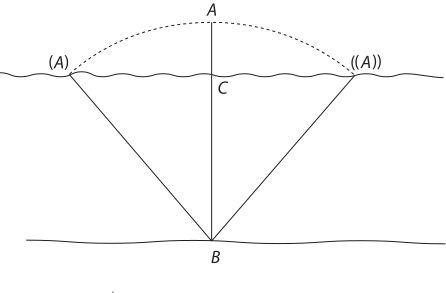
\includegraphics[width=0.7\textwidth]{images/38_139r}
%               \end{center}
            \pstart Soit le plan de l'eau, \textit{(A)((A))} le bâton \textit{AB} fich\'{e} perpendiculairement dans le fonds de l'eau \textit{B} et dont la partie \textit{AC} sorte hors de l'eau. Remuez le bâton, sans 
            le tirer pourtant, et en laissant le bout \textit{B} immobile remuez le, dis je, \`{a} l'entour du centre \textit{B} \edtext{du cost\'{e} gauche}{\lemma{}\Afootnote{du cost\'{e} gauche \textit{ erg.} \textit{ L}}} jusqu'\`{a} ce que le bout \textit{A}, touche l'eau en \textit{(A)}. Faites  la même chose du cost\'{e} droit, jusqu'\`{a} ce que le bout \textit{A} touche l'eau en \textit{((A))}. Ainsi